\documentclass[runningheads]{llncs}
%
\usepackage[T1]{fontenc}
\usepackage{graphicx}
\usepackage{amsfonts,amssymb}
\usepackage{amsmath}         % for matrices in equations
\usepackage{bm}              % bold greeks
\usepackage{xfrac}           % slanted fractions
%\usepackage{algorithm} % <-- needed for standard algorithm float
\usepackage[linesnumbered,ruled]{algorithm2e}
\usepackage [autostyle, english = american]{csquotes} % left and right opening quotes with "
\MakeOuterQuote{"}


% all the following for multiline commands in algorithm2e
\newcommand{\nosemic}{\SetEndCharOfAlgoLine{\relax}}% Drop semi-colon ;
\newcommand{\dosemic}{\SetEndCharOfAlgoLine{\string;}}% Reinstate
\newcommand{\pushline}{\Indp}% Indent
\newcommand{\popline}{\Indm\dosemic}% Undent
\newcommand{\mb}[1]{\text{\boldmath$#1$}}
\newcommand{\gb}[1]{\!\!\text{\boldmath$#1$}\!\!}

\allowdisplaybreaks
\raggedbottom

%
\begin{document}
%
\title{Fore-and-Back for Changepoint Analysis}
%
%\titlerunning{F&B for changepoint anaysis}
\author{Vittorio Maniezzo\inst{1}\orcidID{0000-0002-1220-1235}}

%
\authorrunning{V. Maniezzo}
% First names are abbreviated in the running head.
% If there are more than two authors, 'et al.' is used.
%
\institute{University of Bologna, Cesena, Italy\\
\email{vittorio.maniezzo@unibo.it}\\
\url{https://www.unibo.it/sitoweb/vittorio.maniezzo/en}}
% morteza.sheykhizadeh@studio.unibo.it
\maketitle              % typeset the header of the contribution
%
\begin{abstract}
This paper introduces a novel fore–n–back matheuristic for changepoint detection in univariate time series, combining the modeling rigor of mathematical programming with the efficiency of heuristic search. Classical exact approaches to optimal partitioning, such as dynamic programming, offer strong optimality guarantees but typically exhibit quadratic time and memory requirements in the sequence length, which can limit their applicability to long series or resource-constrained settings.
The proposed method embeds an optimization-based formulation within an iterative forward–backward search scheme that rapidly constructs high-quality feasible segmentations and incrementally improves them as additional computational resources become available. This design yields an anytime algorithm that preserves the structural advantages of exact models—such as extensibility and constraint handling—while avoiding exhaustive exploration.
Computational experiments show that the matheuristic consistently attains near-optimal solutions at a fraction of the computational cost of standard exact methods, providing a scalable and flexible alternative for optimization-based changepoint detection in practice.
\keywords{Changepoint analysis \and matheuristics \and Fore-and-Back.}
\end{abstract}
%
%
%
\section{Introduction}	\label{sec:introducion}
Changepoint detection (CPD) is the problem of identifying locations in a time series where the underlying data-generating process changes abruptly. Such changes may correspond to shifts in mean, variance, trend, or more complex structural properties, and their accurate detection is central to a wide range of applications, including industrial process monitoring, finance, bioinformatics, network security, and environmental analysis. As modern sensing and logging technologies generate increasingly long and high-frequency time series, there is a growing demand for CPD methods that are not only statistically sound but also computationally scalable and adaptable to practical constraints.

A common and widely studied formulation of CPD is the optimal partitioning problem, in which the time series is segmented into contiguous intervals so as to minimize a global objective composed of within-segment costs and a penalty on the number of changepoints. This framework encompasses many classical likelihood-based and least-squares models and admits exact solution methods with strong optimality guarantees. Dynamic programming (DP) approaches constitute the canonical exact solution technique for this problem and, when segment costs can be computed efficiently, achieve quadratic time and memory complexity in the length of the series. Despite important advances such as pruning strategies and average-case improvements, these methods may still become computationally demanding for very long sequences, complex segment models, or when additional structural constraints are imposed.

In parallel to algorithmic developments, mathematical programming formulations—typically based on mixed-integer linear or quadratic models—have been proposed to address CPD in a unified optimization framework. These approaches offer several advantages, including modeling flexibility, the ability to incorporate global constraints across segments, and conceptual clarity. However, their direct solution via general-purpose solvers often requires exploring a large combinatorial search space, which can limit their practical applicability, especially in low-latency or resource-constrained environments. As a result, there remains a gap between the expressive power of optimization-based CPD models and the computational efficiency demanded by large-scale or time-critical applications.

Matheuristics, which integrate mathematical programming techniques within heuristic or metaheuristic frameworks, provide a promising avenue for bridging this gap. By leveraging the structural strength of exact models while selectively relaxing exhaustive search, matheuristics aim to deliver high-quality solutions with significantly reduced computational effort. In the context of CPD, however, relatively few approaches explicitly exploit this paradigm, and most existing methods fall either on the side of exact optimization or on purely algorithmic heuristics.

This paper proposes a novel matheuristic for univariate changepoint detection based on a *fore–n–back* search strategy. The method starts from a rapidly generated feasible segmentation and alternates between forward construction and backward refinement phases, guided by an underlying mathematical programming formulation. This design enables the algorithm to quickly identify promising regions of the solution space while retaining a global view of the segmentation problem. Importantly, the approach is *anytime* in nature: it produces a valid solution almost immediately and progressively improves solution quality as additional computational resources become available.

The proposed matheuristic preserves key advantages of optimization-based CPD models. In particular, it naturally supports the inclusion of global constraints on the segmentation, such as bounds on the number of segments or minimum segment lengths, which are difficult to accommodate within classical dynamic programming frameworks. At the same time, by avoiding a full enumeration of candidate segmentations, the method circumvents the computational burden typically associated with exact solvers.

Extensive computational experiments demonstrate that the proposed approach consistently yields near-optimal solutions while requiring only a fraction of the computational effort of standard exact methods. These results suggest that the fore–n–back matheuristic provides an effective compromise between statistical accuracy and runtime efficiency, making it well suited for large-scale and resource-constrained CPD applications.

The remainder of the paper is organized as follows. Section 2 reviews related work on changepoint detection and optimization-based approaches. Section 3 introduces the mathematical programming formulation underlying the proposed method. Section 4 details the fore–n–back matheuristic and its algorithmic components. Section 5 presents computational results, and Section 6 concludes with directions for future research.

\section{Changepoint analysis} 	\label{sec:changepoints}
Letteratura etc. \cite{the_book}

Changepoint detection has been extensively studied across statistics, machine learning, and operations research, leading to a rich body of methodological literature. Early approaches focused on hypothesis testing and likelihood ratio methods applied sequentially or retrospectively, often with limited scalability or weak global optimality guarantees. More recent work has converged on segmentation-based formulations, in which the time series is partitioned into contiguous segments by minimizing a penalized cost function. Comprehensive surveys of this evolution can be found in \cite{AC17} and \cite{TOV20}.

From an algorithmic standpoint, dynamic programming (DP) has emerged as the canonical tool for solving optimal partitioning problems exactly. While classical DP incurs quadratic time and memory complexity, a substantial line of research has focused on pruning strategies to improve practical performance. Notable examples include PELT \cite{KFE12}, functional pruning \cite{R15}, and segment neighborhood methods \cite{AL89}. Although highly effective under favorable conditions, these methods rely on assumptions about the cost structure or penalty function and may lose efficiency when segment costs are complex, constraints are added, or worst-case behavior is encountered.

Beyond exact DP-based approaches, a variety of heuristic and approximate methods have been proposed to address scalability concerns. Binary segmentation and its variants \cite{SK74} \cite{FLS09} iteratively split the series using local test statistics and are computationally efficient, but they are known to suffer from suboptimal global behavior. Wild binary segmentation and related multiscale procedures improve detection power but still lack a global optimization perspective and provide limited control over structural constraints.

Sliding-window and online heuristics, often based on distance or local statistics, have been widely explored for detecting changes very shortly after its occurrence (low-latency detection, e.g., \cite{KCHP01} \cite{KCHP02}). While computationally efficient, such methods typically rely on local information and offer limited control over global segmentation structure.

Optimization-based heuristics form a smaller but growing subset of the CPD literature. Several authors have proposed mixed-integer programming formulations for changepoint detection, highlighting their flexibility and modeling power. However, due to the combinatorial nature of the resulting problems, these formulations are often limited to moderate instance sizes when solved to optimality. To mitigate this issue, relaxation-based methods, warm-start strategies, and restricted search techniques have been explored, though often without a systematic heuristic framework.

Matheuristics offer a principled way to combine the strengths of these two worlds. By embedding mathematical programming models within heuristic search strategies, matheuristics aim to preserve global structure while avoiding exhaustive enumeration. Despite their success in other combinatorial optimization domains, their application to changepoint detection remains relatively underexplored. Existing approaches typically focus either on speeding up exact solvers or on designing problem-specific heuristics, with limited integration between the two.

The method proposed in this paper contributes to this emerging area by introducing a fore–n–back matheuristic that explicitly leverages an optimization-based formulation while maintaining heuristic flexibility and anytime performance. Unlike classical DP or purely algorithmic heuristics, the proposed approach is designed to accommodate complex cost structures and global constraints, positioning it as a complementary alternative within the broader CPD literature.

\section{Fore-and-Back for changepoint analysis}	\label{sec:forenback}
Fore-and-back \cite{BMM08,the_book} is an extension of {\em Beam Search} (BS) that can improve its effectiveness. Fore-and-Back, when run with no limits on computational resources, becomes an exact solution method. However, by design, it is mainly concerned with heuristic solving, trying to quickly get high quality solutions with little attention paid to optimality proofs.

A significant characteristic of this method is that, despite being a primal only method, it is able to compute bounds to the cost of completing partial solutions, therefore to discard partial solutions from expansion and ultimately to reduce the search space.

Beam Search \cite{B08}

\begin{algorithm}
   \SetKwInOut{Input}{Input}
   \SetKwInOut{Output}{Output}
   \SetKw{KwGoTo}{go to}

   \underline{function Fore-and-Back($\delta$, $maxn$, $maxtnodes$)}\;
   \Input{$\delta$, beam width, $maxn$, max total num of nodes, $maxtnodes$, max num of nodes per tree}
   \Output{A feasible solution ${\bf x^*}$ of value $z_{best}$}

   initialize $t=0$, $noimpr = 0$, $nNodes=0$, $z_{best}=\infty$\label{FaB:algo:init}\;
   \While(\tcp*[f]{Alternate forward and backward trees}){$nNodes \leq maxn$}{
      $t=t+1$; $noimpr = noimpr+1$;\

      let $L^t_0 = L_{n+1}^t = \{ \emptyset \}$, $ntNodes$=0\label{FaB:algo:outer_loop}\;
      \ForEach{level $h=1,...,n$}{ \label{FaB:algo:forhloop}
         set $T_h=\{\emptyset\}$;
         \tcp*[f]{generate the node set $T_h$}\\
         \eIf{$t$ is odd}
         {set $k=h$; $k1=h-1$;}
         {set $k=n-h+1$; $k1=n-h+2$;}

         \ForEach(\tcp*[f]{Possible expansions}){node $X \in L^t_{k-1}$}{
            \ForEach{component $s \in S_k$}{
               let $X' = X \cup \{ s \}$\;
               \If{$X'$ meets conditions $i)$ and $ii)$}{
                  set $T_k = T_k \cup X'$\;
                  $ntNodes = ntNodes+1$;\\
                  $nNodes = nNodes+1$;\\
                  \If(\tcp*[f]{feasible solution}){$h = n$ and $c(X') < z_{best}$}{set $z_{best} = c(X')$, $noimpr = 0$ and ${\bf x^*} = X'$;}
               }
            }
            set $E^k = E^k\cup X$;\tcp*[f]{actual node expansion}
         }

         \ForEach(\tcp*[f]{extract the subset $L^t_k \in T_k$}){node $X \in T_k$}{
            \uIf{$\left|T_k\right| \leq \delta$}{
               set $L^t_k = T_k$;
            }
            \Else{
               let $L^t_k$ contain only the $\delta$ least cost partial solutions of $T_k$\;
            }
         }

         \lIf{$ntNodes > maxtnodes$}{\bf break} \label{FaB:algo:goto}
      }
      \lIf(\tcp*[f]{sol. not improved for two iterations}){$noimpr = 2$}{
         $\textbf{stop}$
      }

   }
   \caption{Algorithm Fore-and-Back}
   \label{FaB:peudocode}
\end{algorithm}

In $\text{C++}$, the std::map<int, int> is an excellent choice because it is implemented as a $\text{Red-Black}$ tree, which keeps the keys (your num values) sorted. Store the pairs as std::map<int, int> map name; where the key is num and the value is the minimum cost seen so far for that specific num and all numbers greater than it up to the next existing entry. However, a simpler, more robust approach is to ensure the map only stores non-redundant pairs that form the Pareto frontier of the $(num, cost)$ space.
Operation Standard BBST - std::mapBBST with Pareto Optimization Insert $O(\log N)$ $O(\log N)$ amortized (because dominated elements are permanently removed) Query $O(\log N)$ $O(\log N)$ (for upper bound and decrement)

\section{Computational results}		\label{sec:computational}
Computational results


\paragraph{Sample Heading (Fourth Level)}
The contribution should contain no more than four levels of headings. Table~\ref{tab1} gives a summary of all heading levels.

\begin{table}
	\caption{Table captions should be placed above the
		tables.}\label{tab1}
	\begin{tabular}{|l|l|l|}
		\hline
		Heading level &  Example & Font size and style\\
		\hline
		Title (centered) &  {\Large\bfseries Lecture Notes} & 14 point, bold\\
		1st-level heading &  {\large\bfseries 1 Introduction} & 12 point, bold\\
		2nd-level heading & {\bfseries 2.1 Printing Area} & 10 point, bold\\
		3rd-level heading & {\bfseries Run-in Heading in Bold.} Text follows & 10 point, bold\\
		4th-level heading & {\itshape Lowest Level Heading.} Text follows & 10 point, italic\\
		\hline
	\end{tabular}
\end{table}


Please try to avoid rasterized images for line-art diagrams and schemas. Whenever possible, use vector graphics instead (see Fig.~\ref{fig1}).

\begin{figure}(Ht)
	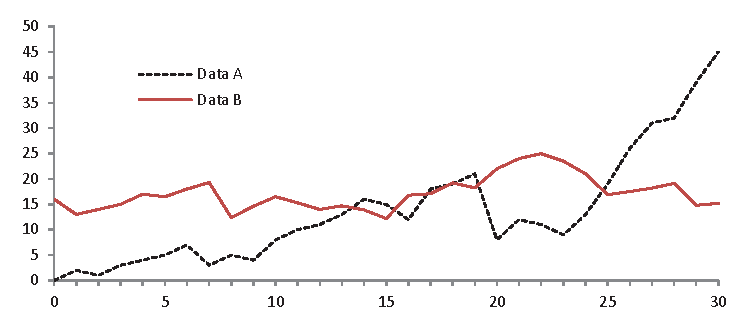
\includegraphics[width=\textwidth]{fig1.eps}
	\caption{A figure caption is always placed below the illustration.
		Please note that short captions are centered, while long ones are
		justified by the macro package automatically.} \label{fig1}
\end{figure}


\section{Conclusions}		\label{sec:conclusions}
The conlusions


\bibliographystyle{splncs04}
\bibliography{LION20_F&B}
\end{document}
